\chapter{Prinzip der rekursiven Definition}\label{ch:Appendix}

\section{Vorwissen für dieses Kapitel}
\subsection{Kartesisches Produkt}
Das folgende Konzept führen wir ein, um über \enquote{Funktionen in mehreren Variablen} sprechen zu können.

Aus zwei Objekten $a$ und $b$ kann ein neues Objekt, das \tib{geordnete Paar}\index{geordnetes Paar} $(a,b)$, gebildet werden. Das erste (zweite) Element des geordneten Paares $(a,b)$ wird erste (zweite) Komponente genannt. Zwei geordnete Paare $(a,b)$ und $(x,y)$ sind genau dann gleich, also $(a,b)=(x,y)$, falls sowohl $a=x$ als auch $b=y$ gelten. Falls $a\neq b$ ist, dann gilt somit auch $(a,b)\neq (b,a)$. Ein geordnetes Paar wird auch \textit{Tupel} genannt.

Seien $A$ und $B$ zwei Mengen. Das \tib{kartesische Produkt}\index{kartesisches Produkt} $A\times B$ von $A$ und $B$ ist diejenige Menge, welche genau aus allen geordneten Paaren $(a,b)$ mit $a\in A$ und $b\in B$ besteht.

\beispiele{-}
{}
{
Wir betrachten die Mengen $A = \lrc{a,b}$ und $B = \lrc{a}$. Dann ist das kartesische Produkt von $A$ und $B$ die Menge
\begin{align*}
    A\times B = \lrc{(a,a), (b,a)}.
\end{align*}
}
{
Seien $A:=\lrc{\text{Marina, Peter, Sandra}}$ und $B:=\lrc{\text{Heidi, Josef}}$ zwei Gruppen (Mengen) von Personen. Jede Person aus Gruppe $A$ tanzt an einem Abend mit jeder Person aus Gruppe $B$ und die Person aus der Gruppe $A$ führt den Tanz an. Dann ist das kartesische Produkt 
\begin{equation*}
\begin{split}
    A\times B = &\{ \text{(Marina, Heidi), (Marina, Josef), (Peter, Heidi)}\\
    &\text{(Peter, Josef), (Sandra, Heidi), (Sandra, Josef)} \}
\end{split}
\end{equation*}
die Menge aller möglichen Tanzpaarungen zwischen Personen aus Gruppe $A$ und Personen aus Gruppe $B$, wobei die Person aus Gruppe $A$ führt. Dabei bedeutet das geordnete Paar $\text{(Marina, Heidi)}$ beispielsweise, dass Marina mit Heidi tanzt (und umgekehrt) und Marina den Tanz führt.
}

\noindent
Das kartesische Produkt dreier Mengen $A, B$ und $C$ wird definiert durch:
\begin{align*}
    A\times B\times C := (A\times B)\times C.
\end{align*}
Ein Element $((a,b),c)$ aus $A\times B\times C$ wird dann allerdings einfach $(a,b,c)$ geschrieben. Dieses Verknüpfen mit weiteren Produkten kann wiederholt\footnote{siehe \cref{sec:rekursion}} werden, um Produkte mit $n$ Faktoren $A_1\times\ldots\times A_n$ (Mengen) zu definieren:
\begin{align*}
    A_1\times\ldots\times A_n := \lr{A_1\times\ldots\times A_{n-1}}\times A_n.
\end{align*}
Für ein Element $a\in\lr{A_1\times\ldots\times A_n}$ schreiben wir nicht etwa $(\ldots (((a_1,a_2),a_3),a_4),\ldots, a_n)$, sondern lediglich $(a_1,\ldots, a_n)$ und nennen $a$ ein \tib{$n$-Tupel}\index{Tupel}.

Ist $X$ eine Menge, dann bezeichnen wir das kartesische Produkt
\begin{align*}
    \underbrace{X\times \ldots \times X}_{n\text{-mal der Faktor }X},
\end{align*}
indem der Faktor $X$ $n$-mal vorkommt, mit $X^n$.

\beispiel{-}{
Die Position eines geometrischen Punktes $P$ im zweidimensionalen Raum (der Ebene) ist eindeutig bestimmt durch zwei Raumkoordinaten. Die beiden Raumkoordinaten des Punktes $P$ in \cref{fig:ebene} sind 2 und 3. Die Ebene können wir uns also denken als die Menge aller Punkte mit Koordinaten der Form $(x,y)$, wobei $x$ und $y$ jeweils reelle Zahlen sind. Somit können wir die Ebene mit dem kartesischen Produkt $\R^2 := \R\times\R$ identifizieren.
\begin{figure}[H]
\begin{center}
\begin{tikzpicture}[scale=0.7]
    \begin{scope}[thick,font=\scriptsize]
    \draw [dashed, very thin] (2,0) -- (2,3);
    \draw [dashed, very thin] (0,3) -- (2,3);
    \draw [thick, -stealth] (-4,0)--(7,0) node[below]{$\R$};
    \draw [thick, -stealth] (0,-4)--(0,7) node[left]{$\R$};
    \foreach \n in {-4,...,-1,1,2,...,4}{%
        \draw (\n,-4pt) -- (\n,4pt)   node [below=0.15cm] {$\n$};
        \draw (-4pt,\n) -- (4pt,\n)   node [left=0.15cm] {$\n$};
    }
    \draw [color=blue, fill=blue] (2,3) circle(0.06);
    \node [color=black] at (3.1,3) {$P = (2,3)$};
\end{scope}
\end{tikzpicture}
\end{center}
\caption{geometrische Interpretation des 2-Tupels $P = (2,3)$ als geometrischer Punkt in der Ebene}
\label{fig:ebene}
\end{figure}
\noindent
Analog können wir den dreidimensionalen Raum mit dem kartesischen Produkt $\R\times\R\times\R := \R^3$ identifizieren.
}

\subsection{Neue Sichtweise auf Funktionen}
Wir betrachten nochmals \cref{definition:funktion}. Dort haben wir gesagt, dass eine Funktion auf einer Menge $X$ mit Werten in $Y$ definiert ist, wenn eine Vorschrift (Regel) $f$ existiert, die jedem Element $x\in X$ genau eine Zahl $y\in Y$ zuordnet. Diese Definition ist sehr anschaulich und nützlich. Nun ist allerdings aus Sicht der Mathematik nicht ganz klar, was mit einer \textit{Vorschrift} oder \textit{Regel} gemeint ist. Um den Begriff der Funktion zu präzisieren, müssen die Definitionsmenge $X$ und die Zielmenge $Y$ miteinander in geeigneter Weise verknüpft werden. Es stellt sich heraus, dass das kartesische Produkt $X\times Y$ eine solche geeignete Verknüpfung darstellt. Beachten Sie, dass das kartesische Produkt $X\times Y$ selbst wiederum eine Menge ist. Die etwas vagen Begriffe der \textit{Vorschrift} oder \textit{Regel} können mit Hilfe des kartesischen Produkts ganz genau festgehalten werden. Beachten Sie, dass eine Funktion $f$ mit $f: X\to Y$ jedem Element $x\in X$ genau ein Element $y\in Y$ zuordnet. Dies bedeutet, dass für alle $x\in X$, falls $f(x)=y_1$ und gleichzeitig $f(x)=y_2$ gelten, stets folgen muss, dass $y_1=y_2$. Dies muss so sein, denn sonst würde einem Element $x\in X$ nicht genau ein $y\in Y$ zugeordnet werden. Damit wäre aber $f$ keine Funktion.

\beispiel{beispiel:relation}
{
Seien $X$ und $Y$ die folgenden Mengen:
\begin{align*}
    X := \lrc{Eric, Stan, Kyle, Kenny}, \quad Y := \lrc{E, I, G}.
\end{align*}
Dabei stehen $E, I$ und $G$ für die Wahlfächer \textbf{E}nglisch, \textbf{I}nformatik und \textbf{G}eschichte.
Das kartesische Produkt $X\times Y$ ist dann die folgende Menge mit 12 Elementen:
\begin{equation*}
    \begin{split}
    X\times Y &= \\
    &\{ (Eric, E),(Eric, I),(Eric, G),(Stan, E),(Stan, I),(Stan, G),\\
    &(Kyle, E),(Kyle, I),(Kyle, G),(Kenny, E),(Kenny, I),(Kenny, G) \}.
    \end{split}
\end{equation*}
Intuitiv hat die Menge $X\times Y$ in diesem Beispiel die Bedeutung, dass jeder der vier Jungen jeweils jedes der drei Wahlfächer wählt. Jeder Junge steht also in Beziehung zu jedem der Fächer. Nun sind natürlich auch noch diverse andere Beziehungen zwischen den Jungen und den Wahlfächern denkbar. So hat beispielsweise die Teilmenge
\begin{align*}
    \lrc{(Stan, E), (Stan, G)} \subseteq X\times Y
\end{align*}
von $X\times Y$ die Bedeutung, dass Stan genau die beiden Wahlfächer Englisch und Geschichte wählt und die anderen drei Jungen jeweils kein Wahlfach wählen. Es ist intuitiv klar, dass jede Teilmenge von $X\times Y$ eine Form von Beziehung zwischen den Jungen und den Wahlfächern darstellt. Eine solche Beziehung wird in der Mathematik eine \textit{Relation} zwischen $X$ und $Y$ genannt (siehe \cref{definition:relation}). 

Nun stellt eine Funktion von $X$ nach $Y$ eine spezielle Relation dar. Nicht jede Teilmenge von $X\times Y$ ist eine Funktion von $X$ nach $Y$, aber jede Funktion von $X$ nach $Y$ ist eine Teilmenge von $X\times Y$. Eine Funktion (funktionale Relation) $f$ von $X$ nach $Y$ soll die Eigenschaft haben, dass sie jedem Element $x\in X$ genau ein Element $y\in Y$ zuordnet. Die Teilmengen $X\times Y$ und $\lrc{(Stan, E), (Stan, G)}$ sind also sicherlich keine Funktionen von $X$ nach $Y$, die zwei Teilmengen
\begin{align*}
    &\lrc{(Eric, I), (Stan, I), (Kyle, E), (Kenny, I)}, \\
    &\lrc{(Eric, G), (Stan, G), (Kyle, G), (Kenny, G)}
\end{align*}
von $X\times Y$ aber zum Beispiel schon.

Betrachten wir nun die neuen Mengen
\begin{align*}
    X := \lrc{0,1,2}, \quad Y := \lrc{0,4,6,7}.
\end{align*}
\begin{figure}[H]
    \centering
    \begin{subfigure}[b]{0.30\textwidth}
        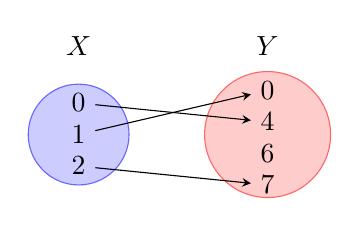
\begin{tikzpicture}[scale=0.8]
            % draw the sets
            \filldraw[fill=blue!20, draw=blue!60] (-1.5,0) circle (0.8cm);
            \filldraw[fill=red!20, draw=red!60] (1.5,0) circle (1cm);
            % the texts
            \node at (-1.5,1.4) {$X$};
            \node at (1.5,1.4) {$Y$};
            % the points in the sets (here I just create nodes to use them later on to position
            % the circles and the arrows
            \node (x1) at (-1.5,0.5) {$0$};
            \node (x2) at (-1.5,0.0) {$1$};
            \node (x3) at (-1.5,-0.5) {$2$};
            
            \node (y1) at (1.5,0.7) {$0$};
            \node (y2) at (1.5,0.2) {$4$};
            \node (y3) at (1.5,-0.3) {$6$};
            \node (y4) at (1.5,-0.8) {$7$};
        
            % draw the arrows
            \draw[-stealth] (x1) -- (y2);
            \draw[-stealth] (x2) -- (y1);
            \draw[-stealth] (x3) -- (y4);
        \end{tikzpicture}
        \caption{eine Funktion}
        \label{subfig:Relation1}
    \end{subfigure}
    \begin{subfigure}[b]{0.30\textwidth}
        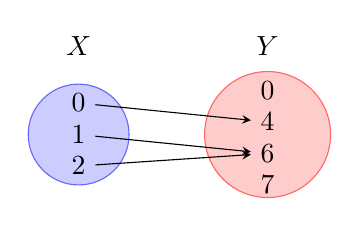
\begin{tikzpicture}[scale=0.8]
            % draw the sets
            \filldraw[fill=blue!20, draw=blue!60] (-1.5,0) circle (0.8cm);
            \filldraw[fill=red!20, draw=red!60] (1.5,0) circle (1cm);
            % the texts
            \node at (-1.5,1.4) {$X$};
            \node at (1.5,1.4) {$Y$};
            % the points in the sets (here I just create nodes to use them later on to position
            % the circles and the arrows
            \node (x1) at (-1.5,0.5) {$0$};
            \node (x2) at (-1.5,0.0) {$1$};
            \node (x3) at (-1.5,-0.5) {$2$};
            
            \node (y1) at (1.5,0.7) {$0$};
            \node (y2) at (1.5,0.2) {$4$};
            \node (y3) at (1.5,-0.3) {$6$};
            \node (y4) at (1.5,-0.8) {$7$};
        
            % draw the arrows
            \draw[-stealth] (x1) -- (y2);
            \draw[-stealth] (x2) -- (y3);
            \draw[-stealth] (x3) -- (y3);
        \end{tikzpicture}
        \caption{ebenfalls eine Funktion}
        \label{subfig:Relation2}
    \end{subfigure}
    \begin{subfigure}[b]{0.30\textwidth}
        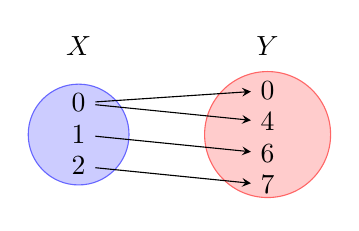
\begin{tikzpicture}[scale=0.8]
            % draw the sets
            \filldraw[fill=blue!20, draw=blue!60] (-1.5,0) circle (0.8cm);
            \filldraw[fill=red!20, draw=red!60] (1.5,0) circle (1cm);
            % the texts
            \node at (-1.5,1.4) {$X$};
            \node at (1.5,1.4) {$Y$};
            % the points in the sets (here I just create nodes to use them later on to position
            % the circles and the arrows
            \node (x1) at (-1.5,0.5) {$0$};
            \node (x2) at (-1.5,0.0) {$1$};
            \node (x3) at (-1.5,-0.5) {$2$};
            
            \node (y1) at (1.5,0.7) {$0$};
            \node (y2) at (1.5,0.2) {$4$};
            \node (y3) at (1.5,-0.3) {$6$};
            \node (y4) at (1.5,-0.8) {$7$};
        
            % draw the arrows
            \draw[-stealth] (x1) -- (y2);
            \draw[-stealth] (x1) -- (y1);
            \draw[-stealth] (x2) -- (y3);
            \draw[-stealth] (x3) -- (y4);
        \end{tikzpicture}
        \caption{keine Funktion}
        \label{subfig:keineRelation}
    \end{subfigure}%
    \caption{schematische Darstellung der Eigenschaften in \cref{definition:eigenschaftenFunktionen}}
    \label{fig:relationen}
\end{figure}
\noindent
In \cref{fig:relationen} sind drei verschiedene Relationen auf $X\times Y$ gezeigt. Zwei davon sind Funktionen und eine nicht.
}

\begin{definition}[Relation]{definition:relation}
    Seien $X$ und $Y$ zwei Mengen. Eine \tib{Relation} $\mathcal{R}$ ist eine Teilmenge des kartesischen Produkts $X\times Y$, also $\mathcal{R}\subseteq X\times Y$. Damit ist eine Relation $\mathcal{R}$ jede Menge geordneter Paare $(x,y)$.
\end{definition}

\begin{definition}[funktionale Relation]{definition:funktionaleRelation}
Eine Relation $\mathcal{R}$ wird \tib{funktional} genannt, falls
\begin{align*}
    (\;(x,y_1)\in\mathcal{R}\;\land\; (x,y_2)\in\mathcal{R}\;) \Rightarrow (y_1=y_2).
\end{align*}
Eine \tib{funktionale Relation} wird als \tib{Funktion} bezeichnet. Falls $X$ und $Y$ zwei (nicht notwendigerweise verschiedene) Mengen sind, ist eine Relation $\mathcal{R}\subseteq X\times Y$ eine funktionale Relation auf $X$, falls für jedes $x\in X$ ein eindeutiges Element $y\in Y$ existiert, sodass $(x,y)\in\mathcal{R}$. Eine derartige funktionale Relation $\mathcal{R}\subseteq X\times Y$ ist eine \tib{Abbildung} \textit{von} $X$ \textit{nach} $Y$ oder eine \tib{Funktion} \textit{von} $X$ \textit{nach} $Y$.
\end{definition}
In \cref{definition:funktion} haben wir eine Funktion $f:X\to Y$ definiert als die Zuweisung eines Elementes $y\in Y$ \quotes{zugehörig} zu $x\in X$ gemäss einer \quotes{Regel} $f$. Wie wir nun sehen, entspricht dies der Relation: Für jedes $x\in X$ existiert ein eindeutiges $y\in Y$, sodass $(x,y)\in f\subseteq X\times Y$. In dieser Betrachtungsweise ist eine Funktion $f: X\to Y$ also eine Teilmenge $f\subseteq X\times Y$ des direkten Produkts ihrer Definitionsmenge $X$ und ihrer Zielmenge $Y$.
\beispiel{-}
{
    Sei $X:=\lrc{1,2,3}$ und $Y:=\lrc{2,3,4}$. Damit enthält das kartesische Produkt $X\times Y$ genau die geordneten Paare
    \begin{align*}
        X\times Y =\lrc{(1,2),(1,3),(1,4),(2,2),(2,3),(2,4),(3,2),(3,3),(3,4)}.
    \end{align*}
    Wir definieren $f$ als die Funktion (funktionale Relation) $f\subseteq X\times Y$, sodass
    \begin{align*}
        f := \setcm{(x,y)\in X\times Y}{y=2x}.
    \end{align*}
    Dann ist $f =\lrc{\textcolor{DarkGreen}{(1,2)},\textcolor{DarkGreen}{(2,4)}}$:
    \begin{align*}
        \begin{matrix*}[r]
            (1,4) & \textcolor{DarkGreen}{(2,4)} & (3,4)\\
            (1,3) & (2,3) & (3,3)\\
            \textcolor{DarkGreen}{(1,2)} & (2,2) & (3,2)\\
        \end{matrix*}
    \end{align*}
    Dies entspricht offensichtlich genau der Beschreibung
    \begin{align*}
        f: X &\to Y,\\
        x &\mapsto 2x
    \end{align*}
einer Ihnen wohlvertrauten linearen Funktion.
}

\noindent
Beachten Sie, dass \cref{definition:funktionaleRelation} durchaus erlaubt, dass die Menge $X$ (Definitionsmenge) oder die Menge $Y$ (Zielmenge) selbst ebenfalls kartesische Produkte von Mengen sind. Tatsächlich tritt dieser Fall häufig und ganz natürlich auf. Betrachten Sie nochmals \cref{fig:ebene}. Eine Vorschrift $f$, welche einem Punkt
\begin{align*}
    P = (x,y)
\end{align*}
der zweidimensionalen Ebene $\R^2 = \R\times\R$ seinen Abstand
\begin{align*}
    \sqrt{x^2 + y^2}
\end{align*}
vom Koordinatenursprung $(0,0)$ zuordnet, ist eine Funktion
\begin{align*}
    f: \R^2 &\to\R,\\
    (x,y) &\mapsto \sqrt{x^2 + y^2}.
\end{align*}
Die Funktion \enquote{nimmt sich einen Punkt} (dies ist ein Element der Ebene $\R^2$) und weist ihm seinen Abstand zum Koordinatenursprung zu (der Abstand ist eine reelle Zahl). Die so definierte Funktion $f$ wird manchmal eine \textit{Funktion in mehreren Variablen} genannt, da der Funktionswert aus mehreren Variablen (in diesem Fall aus zwei) berechnet wird.

\beispiele{-}{}
{Der \textit{Body-Mass-Index} einer Person berechnet sich aus ihrer Körpergrösse $l$ (in Metern) und ihrer Masse $m$ (in Kilogramm) gemäss der Vorschrift
\begin{align*}
    \frac{m}{l^2}.
\end{align*}
Wir lassen hier die physikalischen Einheiten weg und nehmen an, dass $l$ und $m$ reelle Zahlen sind. Dann ist der Body-Mass-Index eine Funktion
\begin{align*}
    \lr{\Rp}\times \lr{\Rp} &\to\R,\\
    (l,m)&\mapsto \frac{m}{l^2}.
\end{align*}
Beachten Sie, dass hier das kartesische Produkt $\lr{\Rp}\times \lr{\Rp} = \lr{\Rp}^2$ der positiven reellen Zahlen mit sich selbst verwendet wurde. Dies ist eine Funktion \enquote{in zwei Variablen $l$ und $m$}.
}
{Wir bezeichnen mit $+$ die Addition in den natürlichen Zahlen. Dann ist $+$ eine Funktion $+: \N\times \N \to\N$. Sie erhält als Eingaben zwei natürliche Zahlen $x,y$ und berechnet ihre Summe $+(x,y)$, welche selbst wieder eine natürliche Zahl ist. Anstelle von $+(x,y)$ schreiben wir aber $x + y$. So gilt beispielsweise $(3,5)\in\N^2$ und
\begin{align*}
    +(3,5) = 3 + 5 = 8 \in\N.
\end{align*}
Natürlich ist analog auch die Multiplikation $\cdot$ in $\N$ eine Funktion der Form $\cdot: \N^2\to\N$. Hier wurde das kartesische Produkt $\N^2$ verwendet. Auch dies ist eine Funktion \enquote{in zwei Variablen (den beiden Summanden)}.
}
{
Ein sich bewegendes Teilchen hält sich in jedem Augenblick (zur Zeit) $t$ in einem Punkt im $(x(t),y(t),z(t))$ des Raums $\R^3 = \R\times \R\times \R$ auf. Dabei ist $x(t)$ die Funktion, welche für jede Zeit $t$ die erste Raumkoordinate ($x$-Koordinate) des Teilchens angibt. Die Funktion $y(t)$ gibt die zweite Raumkoordinate ($y$-Koordinate) zur Zeit $t$ an und $z(t)$ entsprechend die dritte Raumkoordinate ($z$-Koordinate). Daher kann die Bewegung des Teilchens als Funktion (Abbildung) $\gamma: \R\to\R^3$ interpretiert werden, wobei $\R$ die Zeitachse ist und $\R^3$ der dreidimensionale Raum. Dies ist eine Funktion \enquote{in nur einer Variablen (der Zeit)}, deren Zielmenge allerdings der dreidimensionale Raum $\R^3$ ist.
}
{Seien $X$ und $Y$ Mengen. Eine Funktion
\begin{align*}
    f: X^n\to Y
\end{align*}
erhält also $n$ (nicht notwendigerweise verschiedene) Elemente aus $X$ als Eingabe und nimmt Werte in $Y$ an. Dabei müssen Sie sich in Erinnerung rufen, dass
\begin{align*}
    \underbrace{X^n := X\times \ldots \times X}_{n\text{-mal der Faktor }X}.
\end{align*}
Dies ist eine Funktion \enquote{in $n$ Variablen}.}

\begin{definition}[Graph einer Funktion]{definition:graph}
Mit unserer ursprünglichen \cref{definition:funktion} einer Funktion ist der \tib{Graph} einer Funktion $f: X\to Y$ die Teilmenge $\Gamma$ des kartesischen Produkts $X\times Y$, deren Elemente die Gestalt $(x,f(x))$ besitzen. Damit gilt also:
\begin{align*}
    \Gamma := \setcm{(x,y)\in X\times Y}{y = f(x)}.
\end{align*}
In der Definition einer Funktion als funktionale Relation verschwindet offensichtlich die Unterscheidung zwischen der Funktion $f$ und ihrem Graphen $\Gamma$, da definitionsgemäss $f = \Gamma$ gilt.
\end{definition}


\section{Rekursive Definition}\label{sec:rekursion}
Dieser Abschnitt ist extrem anspruchsvoll. Versuchen Sie, zumindest in groben Zügen, zu verstehen, was das Prinzip der rekursiven Definition aussagt.

\noindent
Mit \cref{definition:fac,definition:fibonacci} der Fakultät und der Fibonacci-Folge haben wir bereits zwei wichtige und bekannte Beispiele rekursiver Definitionen kennengelernt. Bei der Fakultät wird $(n+1)!$ aus dem unmittelbaren Vorgänger $n!$ und einer Multiplikation berechnet. Bei der Fibonacci-Folge wird $F_{n+1}$ aus der Summe der beiden Vorgänger $F_{n}$ und $F_{n-1}$ für $n\in\Nunit$ gebildet.
\begin{myBox}{}
    Allgemein kann man sich vorstellen, dass ein rekursiv definierter Wert $f(n+1)$ abhängig von einigen (möglicherweise von allen) Vorgängern aus $\lrc{f(0), f(1),\ldots, f(n)}$ von $f(n+1)$ ist. Somit wird $f(n+1)$ durch eine Funktion berechnet, welche von allen Vorgängern von $f(n+1)$ abhängig sein darf.
\end{myBox}
Ein Ziel dieses Abschnitts ist es, die Vorstellung \enquote{von Vorgängern abhängen} zu präzisieren. Die \textit{Abhängigkeit} eines rekursiv definierten Wertes $f(n+1)$ von Vorgängern aus
\begin{align*}
    \lrc{f(0), f(1),\ldots ,f(n)}
\end{align*}
lässt sich durch Funktionen definieren. Seien die Funktionswerte $f(0), f(1),\ldots ,f(n)$ jeweils Elemente einer Menge $X$. Die Funktion, nennen wir sie $V_{n+1}$, welche $f(n+1)$ aus den $(n+1)$ Vorgängern $f(0), f(1),\ldots , f(n)$ berechnet, erhält also $n+1$ Werte aus $X$ und gibt selbst wieder einen Wert aus $X$ zurück. Somit ist $V_{n+1}$ also eine Funktion von $X^{n+1}$ nach $X$ und formalisiert die \textit{Abhängigkeit} des Wertes $f(n+1)$ von seinen Vorgängern.

\beispiele{beispiele:PrinzipRek}{}
{
Wir betrachten nochmals das Beispiel der Fakultät. Hier ist $X:=\N$ und für jedes $n\in\N$ definieren wir
\begin{align*}
    V_{n+1}: X^{n+1}\to X, \quad \lr{f(0),\ldots,f(n)} \mapsto (n+1)\cdot f(n).
\end{align*}
Die Definition von $V_{n+1}$ besagt, dass der nächste Wert $f(n+1)$ aus dem Vorgänger $f(n)$, multipliziert mit $(n+1)$, gebildet wird. Dies ist doch genau das, was die Fakultät bedeuten soll! Gemäss \cref{satz:Rekursion}, welchen wir in Kürze vorstellen werden, existiert nun eine eindeutige Funktion $f:\N\to\N$, welche gleichzeitig
\begin{renum}
    \item $f(0) = 1$ und
    \item $f(n+1) = V_{n+1}\lr{f(0),\ldots,f(n)} = (n+1)\cdot f(n), \quad n\in\N$
\end{renum}
erfüllt. Die auf diese Weise definierte Funktion $f$ nennen wir die \textit{Fakultät}.
}
{
Wie sieht es mit der Fibonacci-Folge aus? Auch hier ist $X:=\N$ und wir definieren den Startwert
\begin{align*}
    F(0) := 0
\end{align*}
sowie die Funktion $V_{n+1}: X^{n+1}\to X$:
\[
  V_{n+1}\lr{F(0),F(1),\ldots,F(n)} := 
  \begin{cases}
    1, &\text{falls $n = 0$}, \\
    F(n) + F(n-1), &\text{falls $n\in\Nunit$}.
  \end{cases}
\]
Die Definition von $V_{n+1}$ besagt, dass der nächste Wert $F(n+1)$ für $n\in\Nunit$ aus der Summe der beiden Vorgänger $F(n)$ und $F(n-1)$ gebildet wird. Dies entspricht also genau unserer Vorstellung der Fibonacci-Folge. Erneut garantiert uns \cref{satz:Rekursion} die Existenz einer eindeutigen Funktion $F:\N\to\N$, welche gleichzeitig
\begin{renum}
    \item $F(0) = 1$ und
    \item $F(n+1) = V_{n+1}\lr{F(0),F(1),\ldots,F(n)}, \quad n\in\N$
\end{renum}
erfüllt. Die so definierte Funktion $F$ heisst \textit{Fibonacci-Folge}.
}
{
Es sei $\odot$ eine assoziative Verknüpfung auf einer Menge $X$ und $(x_n)$ eine Folge in $X$. Dann definieren wir für jede natürliche Zahl $n$
\begin{align*}
    \bigodot_{k=0}^{n} := x_0\odot x_1\odot \ldots \odot x_n.
\end{align*}
Diese Definition ist streng mathematisch gesehen nicht sinnvoll, da nicht geklärt ist, was die Bedeutung der drei Punkte auf der rechten Seite ist. Das Prinzip der rekursiven Definition schafft hier Klarheit. Dazu definieren wir für jedes $n\in\N$
\begin{align*}
    V_{n+1}: X^{n+1}\to X, \quad \lr{f(0),\ldots,f(n)} \mapsto x_{n+1}\odot f(n).
\end{align*}
Setzen wir $f(0) = x_0$ sowie
\begin{align*}
    f(n+1) = V_{n+1}\lr{f(0),\ldots, f(n)} = x_{n+1}\odot f(n), \quad n\in\N
\end{align*}
und definieren das Symbol $\bigodot_{k=0}^{n}$ durch
\begin{align*}
    \bigodot_{k=0}^{n} := f(n), \quad n\in\N,
\end{align*}
dann ergibt sich die rekursive Definition
\begin{align*}
    \bigodot_{k=0}^0 = x_0, \quad \bigodot_{k=0}^{n+1} = x_{n+1}\odot \bigodot_{k=0}^{n}x_k, \quad n\in\N.
\end{align*}
Ist mit der assoziativen Verknüpfung $\odot$ die Addition $+$ gemeint, so definieren wir die Summe
\begin{align}\label{eq:summe}
    \sum_{k=0}^n x_k := x_0 + x_1 + \ldots + x_n.
\end{align}
Ist mit der assoziativen Verknüpfung $\odot$ die Multiplikation $\cdot$ gemeint, so definieren wir durch
\begin{align*}
    \prod_{k=0}^n x_k := x_0 \cdot x_1 \cdot \ldots \cdot x_n
\end{align*}
ein Produkt.
}
\noindent
Nun sind wir bei dem in den Beispielen \ref{beispiele:PrinzipRek} bereits mehrfach erwähnten \cref{satz:Rekursion} angelangt. Der Satz formalisiert alle unsere bisherigen Betrachtungen zum Thema der \tib{rekursiven Definition}\index{rekursive Definition} und beschreibt ganz präzise, was wir unter \textit{Rekursion} verstehen wollen.

\begin{satz}[Prinzip der rekursiven Definition]{satz:Rekursion}
Es sei $X$ eine Menge und $a$ ein Element von $X$. Zu jedem $n\in\N$ sei eine Funktion $V_{n+1}: X^{n+1}\to X$ gegeben. Dann existiert genau eine Funktion $f:\N\to X$ mit folgenden Eigenschaften:
\begin{renum}
    \item $f(0) = a$,
    \item für $n\in\N$ gilt $f(n+1) = V_{n+1}\lr{f(0),f(1),\ldots,f(n)}$.
\end{renum}
\end{satz}
\beweis{
\begin{aenum}
\item Zunächst beweisen wir, dass es nur eine solche Funktion geben kann. Angenommen es existieren zwei Funktionen $f,g:\N\to X$, welche jeweils die beiden Eigenschaften des Satzes erfüllen. Es gelte also $f(0) = a$ und $g(0) = a$ sowie für jedes $n\in\N$:
\begin{align}\label{eq:BeweisRekursion}
\begin{split}
    f(n+1) &= V_{n+1}\lr{f(0),f(1),\ldots,f(n)}, \\
    g(n+1) &= V_{n+1}\lr{g(0),g(1),\ldots,g(n)}.
\end{split}
\end{align}
Um zu beweisen, dass $f$ und $g$ identisch sind und somit $f$ eindeutig ist, genügt es nachzuweisen, dass $f(n) = g(n)$ für alle natürlichen Zahlen $n$ gilt. Dieser Nachweis erfolgt durch starke Induktion. Wegen der Eigenschaft $f(0)=g(0)=a$ gilt die Aussage für $n=0$. Dies liefert den Induktionsanfang. Wir zeigen nun, dass aus der Richtigkeit der Aussage $f(k)=g(k)$ für $0\leq k\leq n$ die Richtigkeit der Aussage $f(k+1)=g(k+1)$ folgt. Wegen $\textcolor{Green}{f(k)}=\textcolor{Green}{g(k)}$ für $0\leq k\leq n$ können die Gleichungen \ref{eq:BeweisRekursion} umgeschrieben werden zu:
\begin{align*}
    f(n+1) &= V_{n+1}\lr{\textcolor{Green}{f(0)},\textcolor{Green}{f(1)},\ldots,\textcolor{Green}{f(n)}}, \\
    g(n+1) &= V_{n+1}\lr{\textcolor{Green}{f(0)},\textcolor{Green}{f(1)},\ldots,\textcolor{Green}{f(n)}}.
\end{align*}
Damit hat die Funktion $V_{n+1}$ zweimal dieselben Argumente und somit muss auch 
\begin{align*}
    f(n+1)=g(n+1)
\end{align*}
gelten. Dies beweist den Induktionsschritt.
\item\label{itemb} Wir beginnen den Beweis der Existenz einer solchen Funktion $f$ mit einem vorbereitenden Schritt. Wir behaupten, dass es zu jedem $n\in\N$ eine Funktion
\begin{align*}
    f_n:\lrc{0,1,\ldots,n}\to X
\end{align*}
gibt mit
\begin{align}\label{eq:001}
    f_n(0) &= a, \nonumber\\
    f_n(k) &= f_k(k), \\
    f_n(k+1) &= V_{k+1}\lr{f_n(0),\ldots, f_n(k)}, \nonumber
\end{align}
wobei $k$ eine natürliche Zahl ist, die $0\leq k < n$ erfüllt. Diese Behauptung beweisen wir durch vollständige Induktion. Da es gar keine natürliche Zahl $k$ mit $0\leq k < 0$ gibt, ist die Aussage für $n=0$ offensichtlich richtig. Sei nun die Behauptung für ein $n\in\N$ wahr. Für den Induktionsschritt von $n\to n+1$ definieren wir:
\begin{align*}
    f_{n+1}(k) :=
    \begin{cases}
    f_n(k), &\text{falls $0\leq k\leq n$}, \\
    V_{n+1}\lr{f_n(0),\ldots,f_n(n)}, &\text{falls $k=n+1$}.
    \end{cases}
\end{align*}
Gemäss der Induktionsvoraussetzung gilt für $k\in\N$ mit $0\leq k\leq n$:
\begin{align*}
    f_{n+1}(k) = f_n(k) = f_k(k)
\end{align*}
sowie
\begin{align*}
    &f_{n+1}(k+1) = \\
    &f_n(k+1) = \\
    &V_{k+1}\lr{f_n(0),\ldots, f_n(k)} = \\
    &V_{k+1}\lr{f_{n+1}(0),\ldots, f_{n+1}(k)}
\end{align*}
für $0<k+1\leq n$. Des Weiteren gilt
\begin{align*}
    f_{n+1}(n+1) = V_{n+1}\lr{f_n(0),\ldots, f_n(n)} = V_{n+1}\lr{f_{n+1}(0),\ldots, f_{n+1}(n)}.
\end{align*}
Dies beweist den Induktionsschritt $n\to n+1$ und zeigt die Existenz der Funktionen $f_n$ für alle $n\in\N$ gemäss den Gleichungen \ref{eq:001}.
\item Nach dem vorbereitenden Schritt in Punkt \ref{itemb} definieren wir $f:\N\to X$ durch
\begin{align*}
    f(n) :=
    \begin{cases}
    a, &\text{falls $n=0$}, \\
    f_n(n), &\text{falls $n\in\Nunit$}
    \end{cases}
\end{align*}
und finden
\begin{align*}
    &f(n+1) = \\
    &f_{n+1}(n+1) = \\
    &V_{n+1}\lr{f_{n+1}(0),\ldots,f_{n+1}(n)} = \\
    &V_{n+1}\lr{f_0(0),\ldots,f_n(n)} = \\
    &V_{n+1}\lr{f(0),\ldots,f(n)}.
\end{align*}
\end{aenum}
Somit ist das Prinzip der rekursiven Definition bewiesen. \cite{AmannEscher1}
}

\noindent
Die Tatsache, dass sich das Prinzip der rekursiven Definition (\cref{satz:Rekursion}) in solch direkter Weise durch die vollständige Induktion beweisen lässt, illustriert, wie ähnlich diese Prinzipien sind. Das Prinzip der rekursiven Definition ist eine Folgerung des Induktionsprinzips. Dieses wiederum ergibt sich aus den Peano-Axiomen der natürlichen Zahlen.


% \clearpage
% \shipoutAnswer